
 \begin{figure}[htbp] \begin{center} 
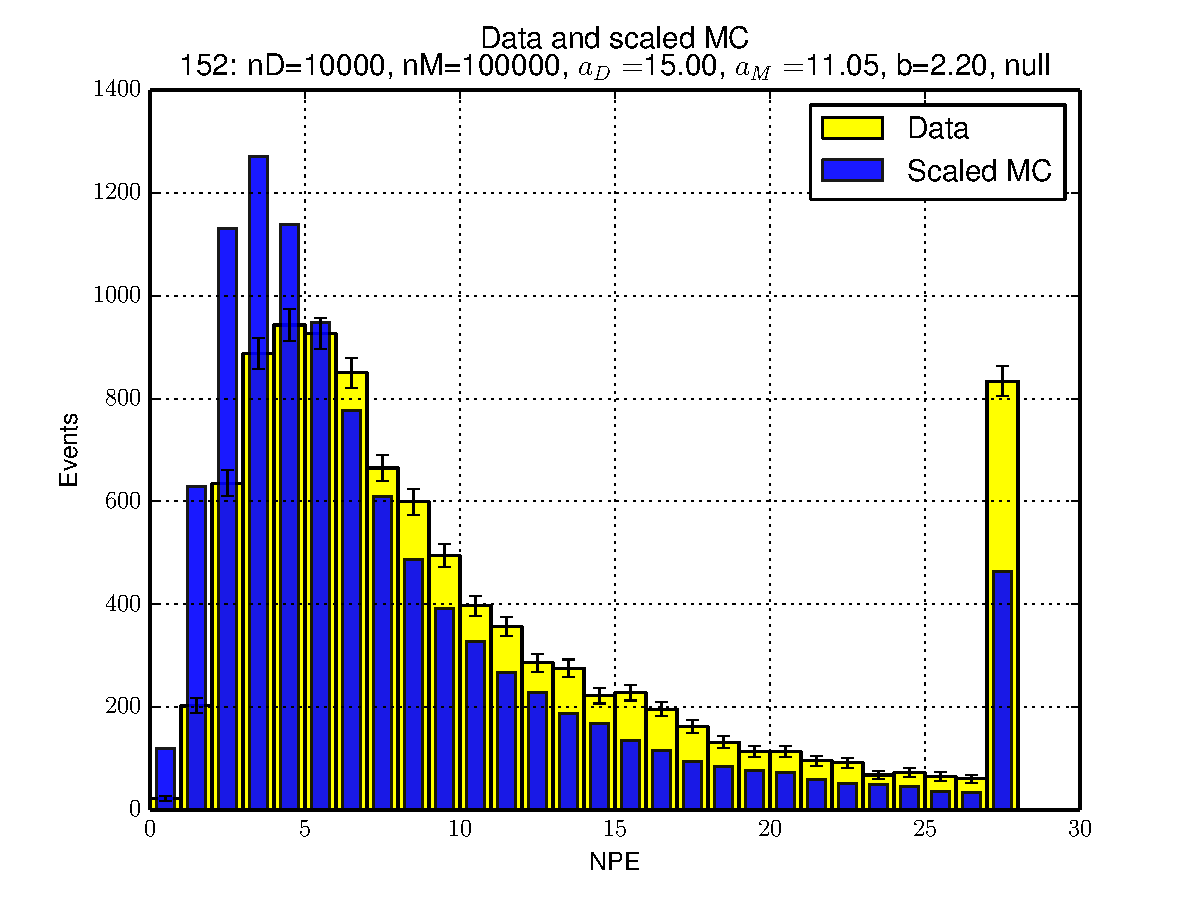
\includegraphics[width=0.45\textwidth]{../FIGURES/152/FIG_Data_and_scaled_MC.pdf} 
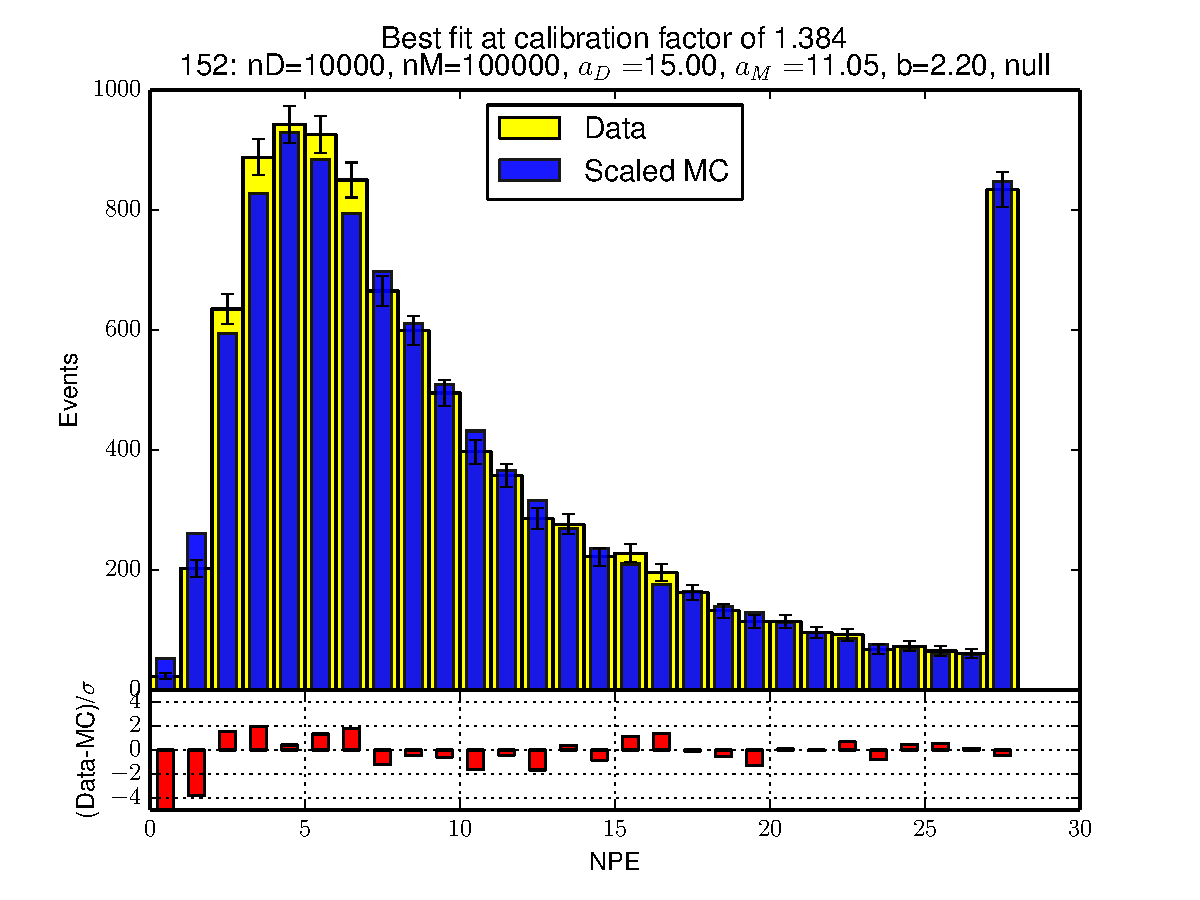
\includegraphics[width=0.45\textwidth]{../FIGURES/152/FIG_Best_fit_at_calibration_factor_of_1_384.pdf} 
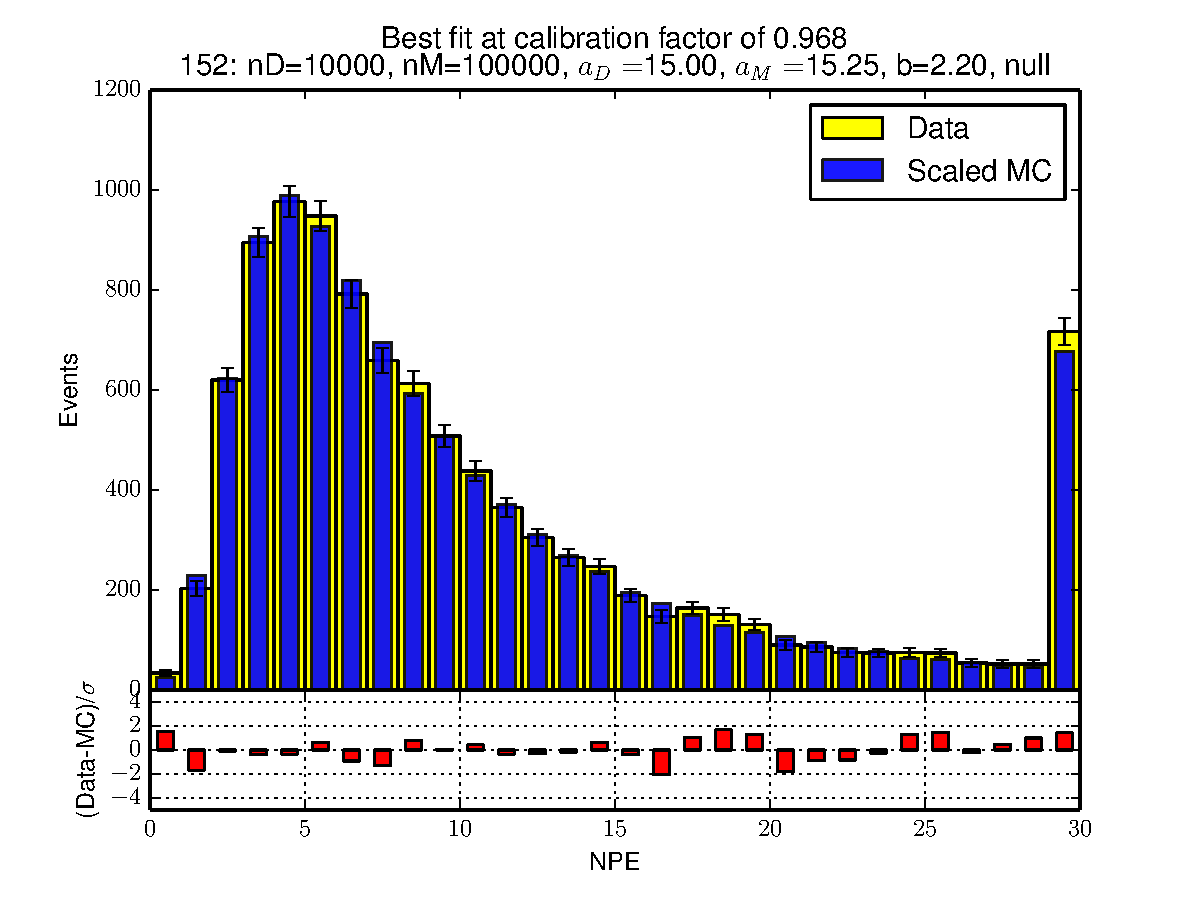
\includegraphics[width=0.45\textwidth]{../FIGURES/152/FIG_Best_fit_at_calibration_factor_of_0_968.pdf} 
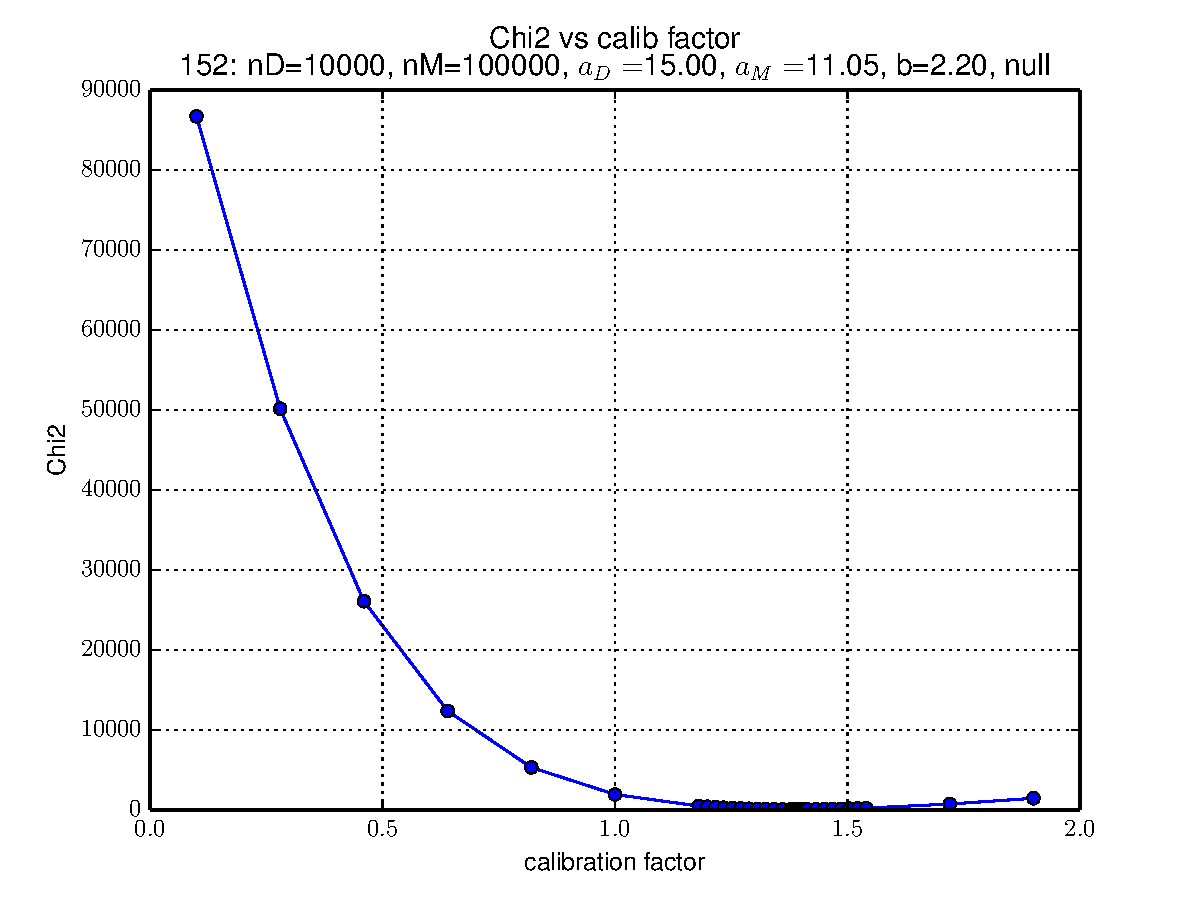
\includegraphics[width=0.45\textwidth]{../FIGURES/152/FIG_Chi2_vs_calib_factor.pdf} 
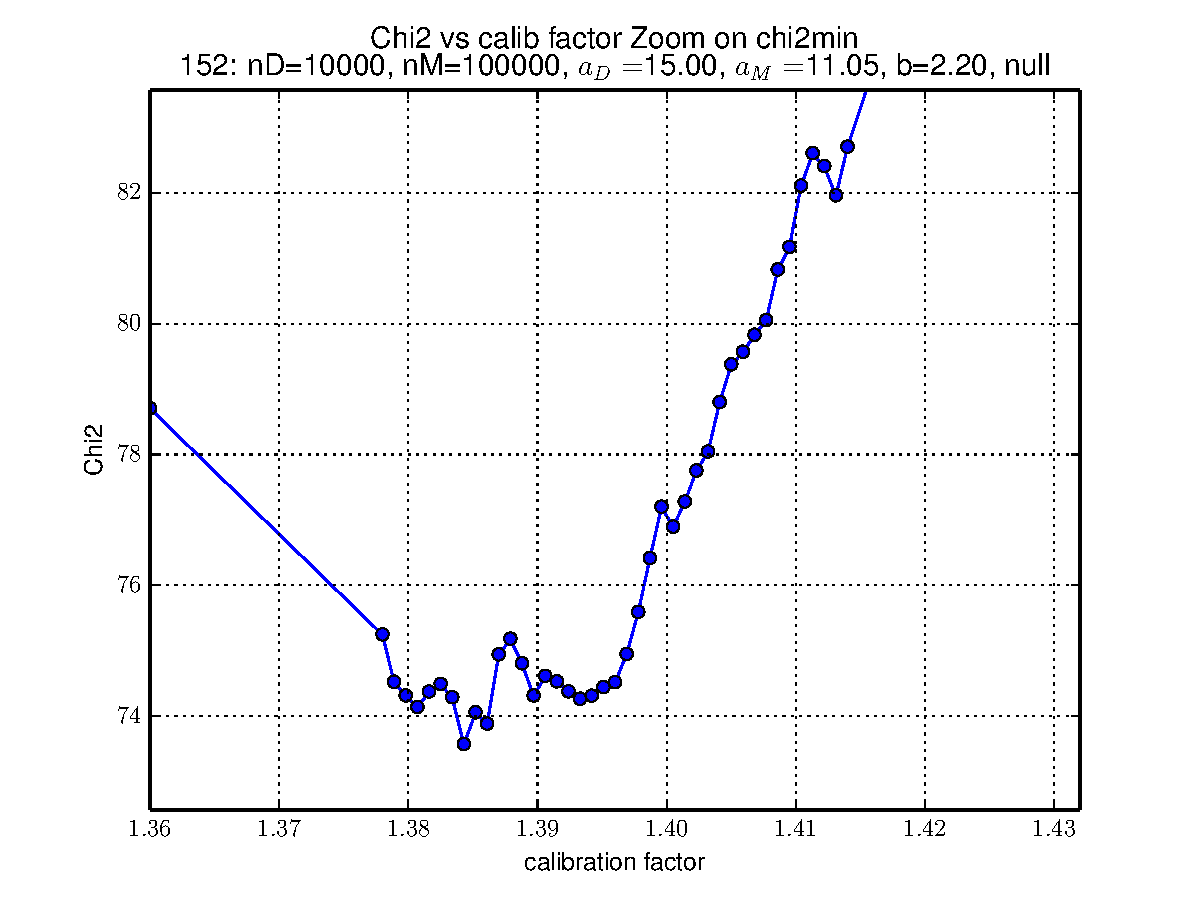
\includegraphics[width=0.45\textwidth]{../FIGURES/152/FIG_Chi2_vs_calib_factor_Zoom_on_chi2min.pdf} 
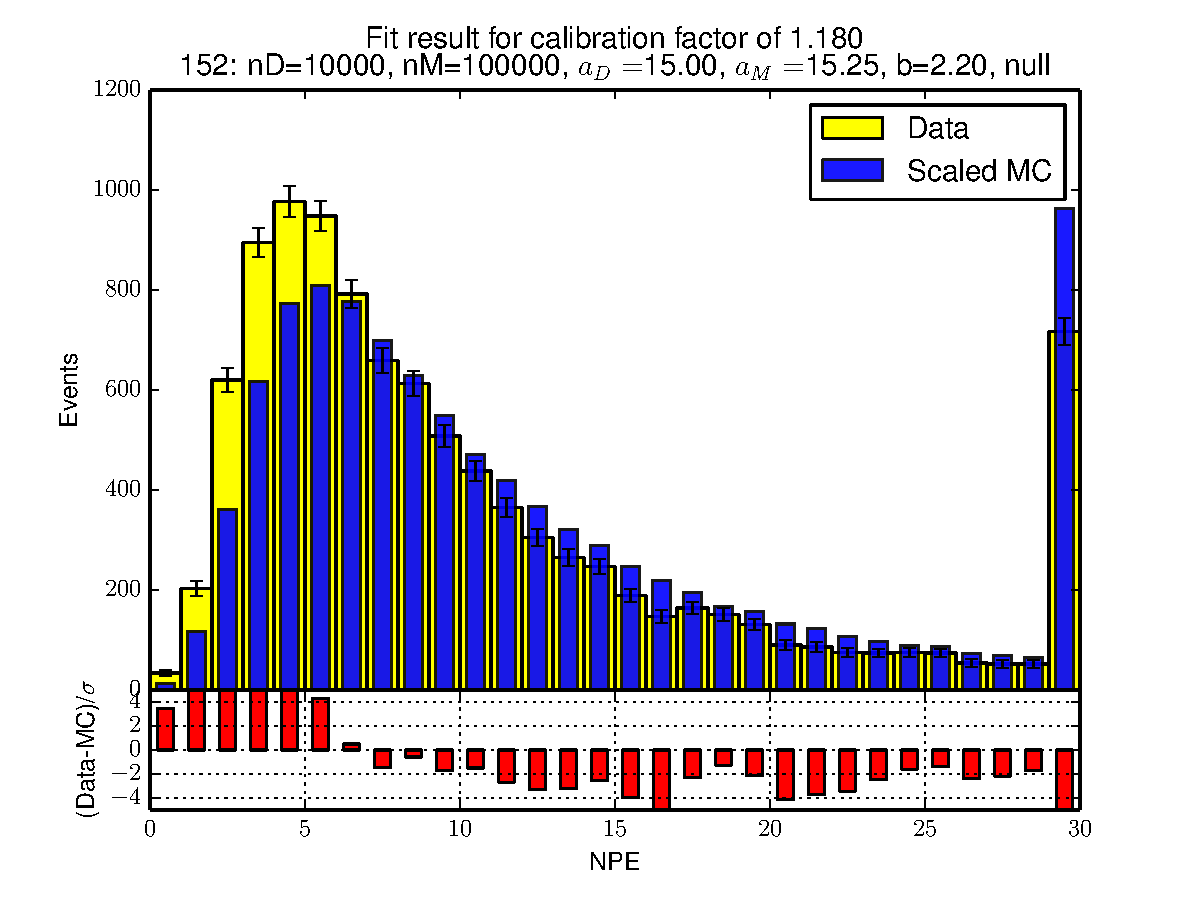
\includegraphics[width=0.45\textwidth]{../FIGURES/152/FIG_Fit_result_for_calibration_factor_of_1_180.pdf} 
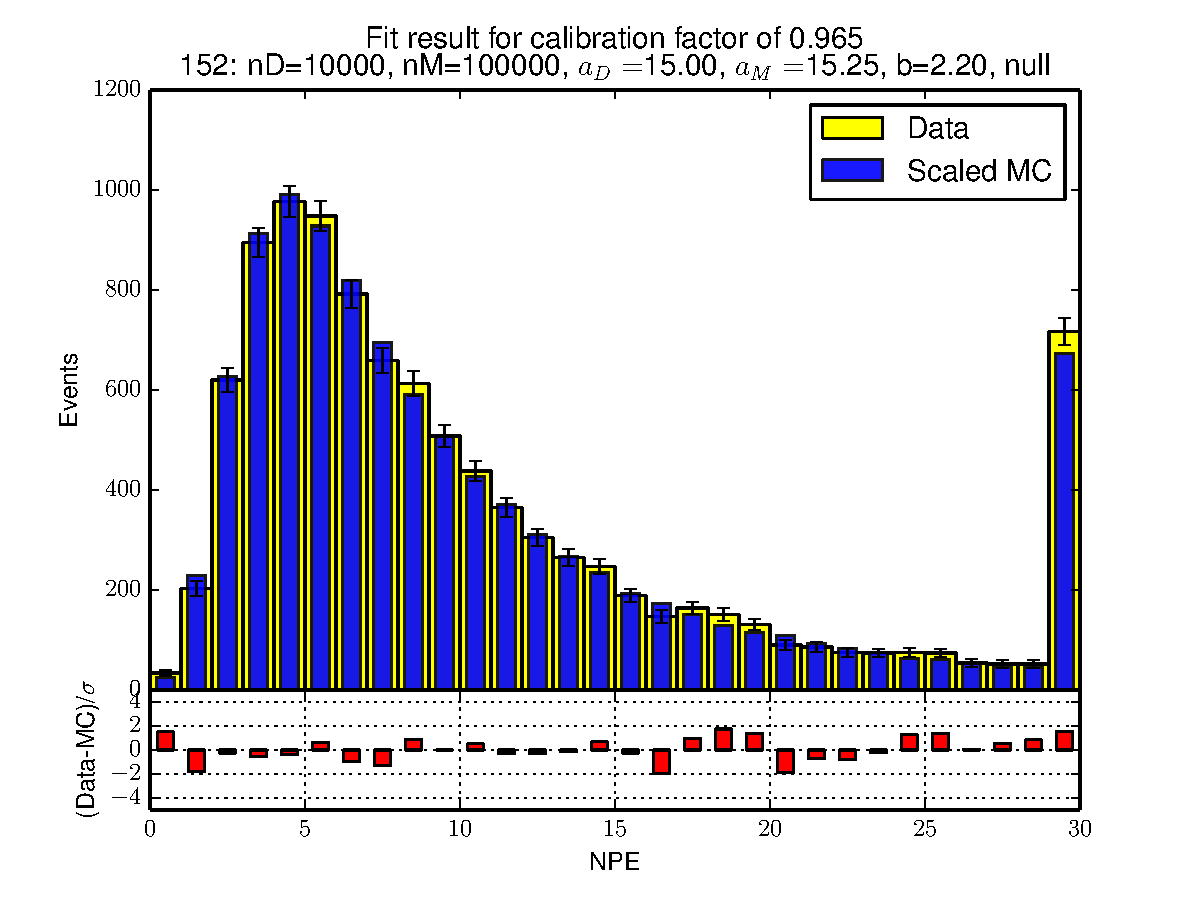
\includegraphics[width=0.45\textwidth]{../FIGURES/152/FIG_Fit_result_for_calibration_factor_of_0_965.pdf} 
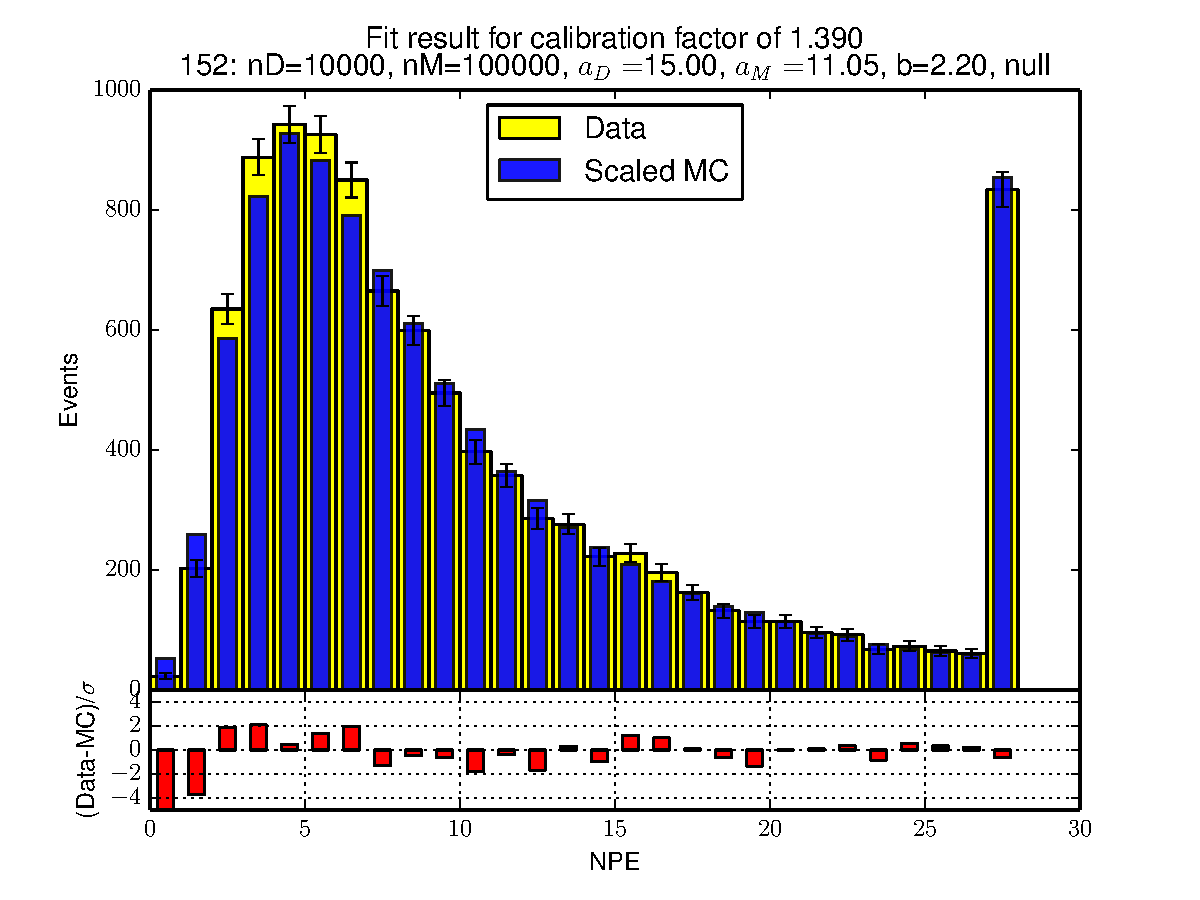
\includegraphics[width=0.45\textwidth]{../FIGURES/152/FIG_Fit_result_for_calibration_factor_of_1_390.pdf} 
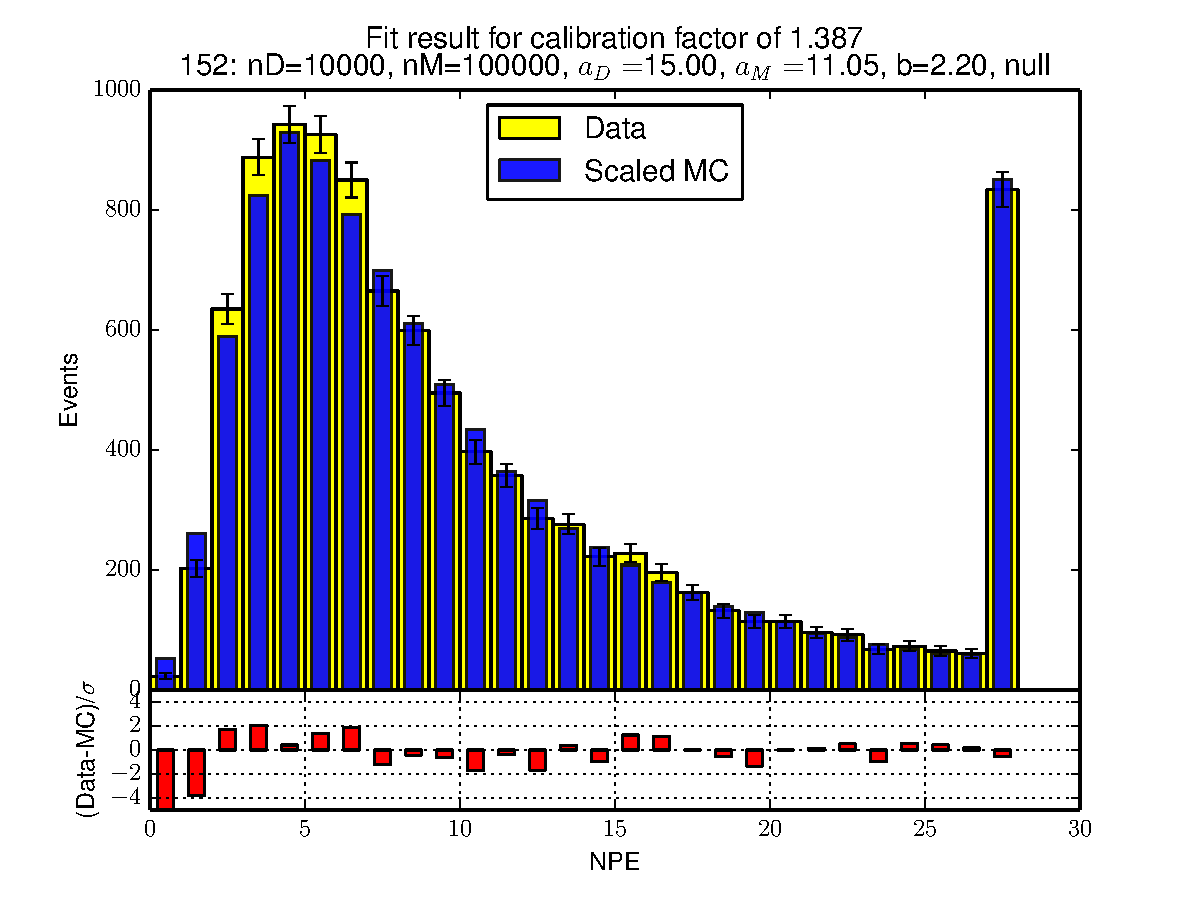
\includegraphics[width=0.45\textwidth]{../FIGURES/152/FIG_Fit_result_for_calibration_factor_of_1_387.pdf} 
\caption{Data compared to nominal MC, MC scaled by the best fit calibration factor, scans of $\chi^2$ over a large range and about the minimum for configuration 152. Data compared to MC scaled by two randomly chosen calibration factors.} 
\label{tab:best_152} 
\end{center} \end{figure} 

 \begin{figure}[htbp] \begin{center} 
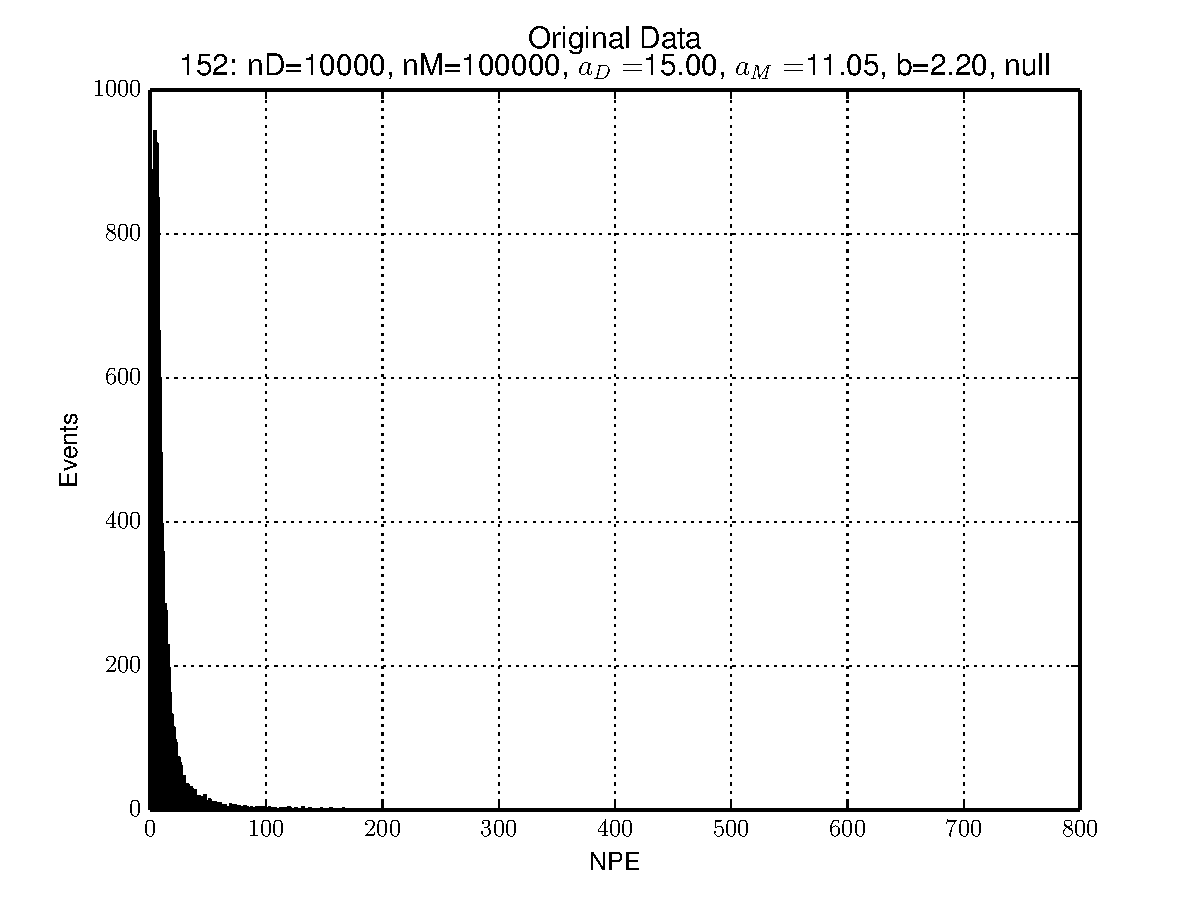
\includegraphics[width=0.45\textwidth]{../FIGURES/152/FIG_Original_Data.pdf} 
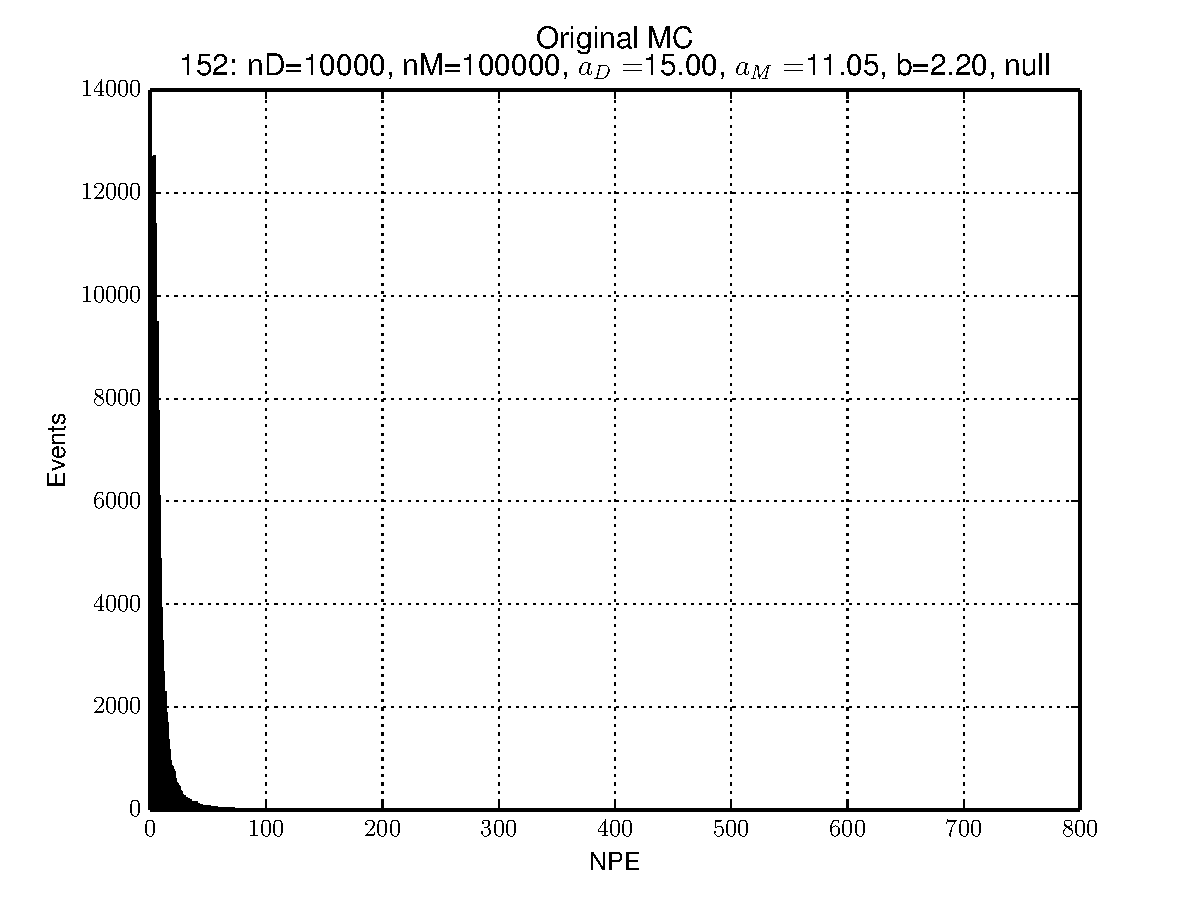
\includegraphics[width=0.45\textwidth]{../FIGURES/152/FIG_Original_MC.pdf} 
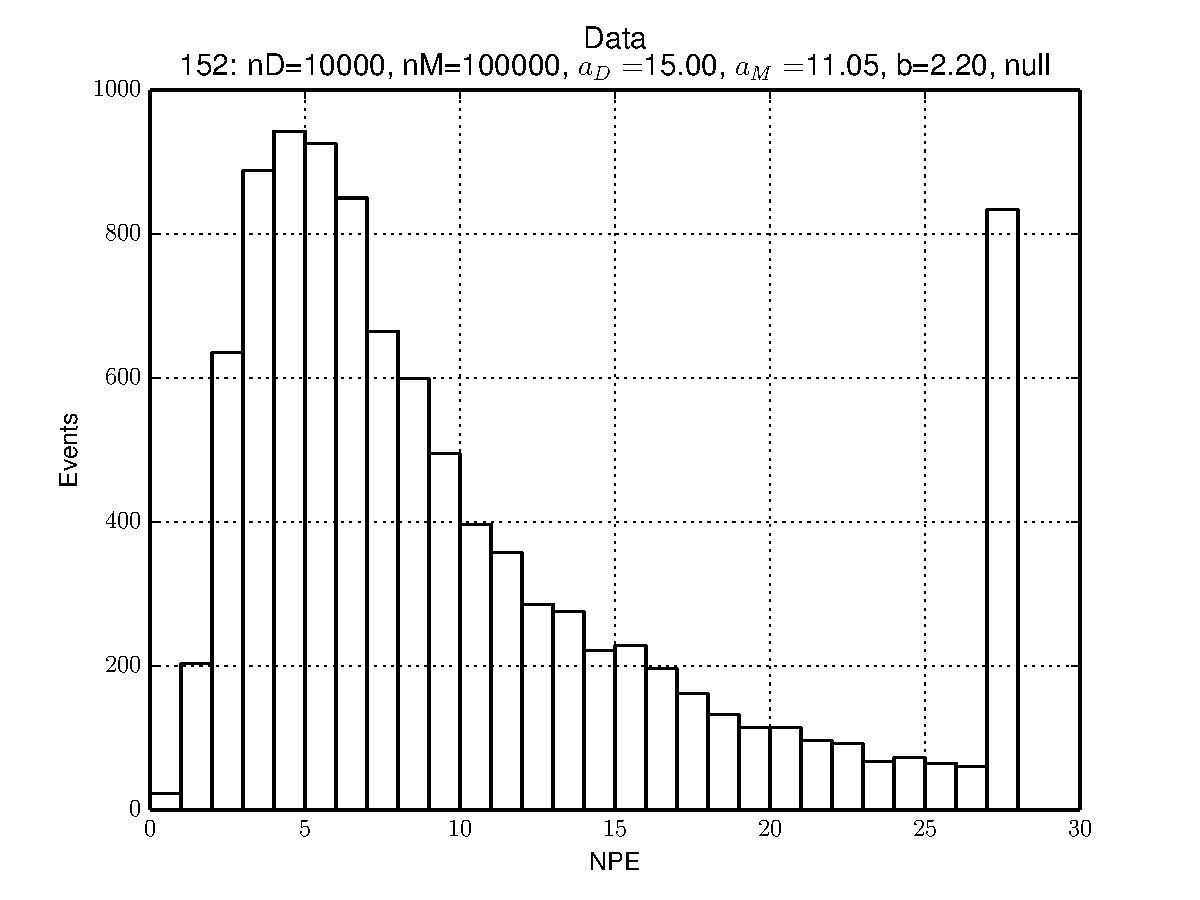
\includegraphics[width=0.45\textwidth]{../FIGURES/152/FIG_Data.pdf} 
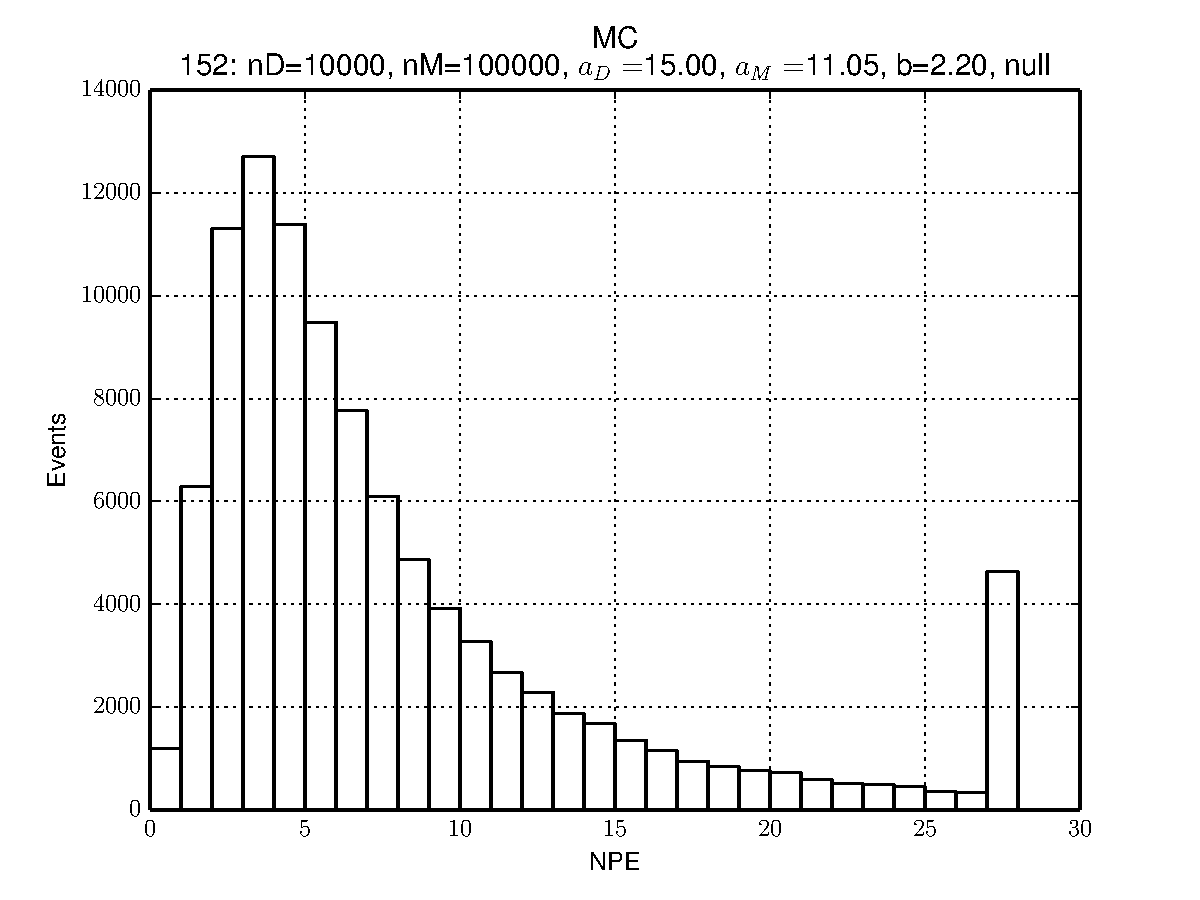
\includegraphics[width=0.45\textwidth]{../FIGURES/152/FIG_MC.pdf} 
\caption{NPE histograms for data and MC for configuration 152. Top are original hists. Bottom are hists after truncation at bin containing less than 10 entries with that bin containing overflows.} 
\label{tab:npe_152} 
\end{center} \end{figure} 
\clearpage
 